%% The first command in your LaTeX source must be the \documentclass command. This is the generic manuscript mode required for submission and peer review.
\documentclass[manuscript,screen,review]{acmart}
%% To ensure 100% compatibility, please check the allowlist of
%% approved LaTeX packages to be used with the Master Article Template at
%% https://www.acm.org/publications/taps/whitelist-of-latex-packages 
%% before creating your document. The allowlist page provides 
%% information on how to submit additional LaTeX packages for 
%% review and adoption.
%% Fonts used in the template cannot be substituted; margin 
%% adjustments are not allowed.

%%
%% \BibTeX command to typeset the BibTeX logo in the docs
\AtBeginDocument{%
  \providecommand\BibTeX{{%
    \normalfont B\kern-0.5em{\scshape i\kern-0.25em b}\kern-0.8em\TeX}}}

%% Rights management information. This information is sent to you
%% when you complete the rights form. These commands have SAMPLE
%% values in them; it is your responsibility as an author to replace
%% the commands and values with those provided to you when you
%% complete the rights form.
\setcopyright{acmcopyright}
\copyrightyear{2024}
\acmYear{2024}
\acmDOI{XXXXXXX.XXXXXXX}




%%
%% Submission ID.
%% Use this when submitting an article to a sponsored event. You'll
%% receive a unique submission ID from the organizers
%% of the event and this ID should be used as the parameter for this command.
%%\acmSubmissionID{123-A56-BU3}

%%
%% For managing citations, it is recommended to use a bibliography
%% files in BibTeX format.
%%
%% You can then either use BibTeX with the ACM-Reference-Format style,
%% or BibLaTeX with the acmnumeric or acmauthoryear styles that include
%% support for advanced citation of software artifact from the
%% biblatex-software package, also separately available on CTAN.
%%
%% Look at the sample-*-biblatex.tex files for templates showcasing
%% the biblatex styles.
%%

%%
%% The majority of ACM publications use numbered citations and
%% references. The command \citestyle{authoryear} switches to the
%% "author year" style.
%%
%% If you are preparing content for an event
%% sponsored by ACM SIGGRAPH, you must use the "author year" style of
%% citations and references.
%% Uncommenting
%% The next command will enable that style.
%%\citestyle{acmauthoryear}

%%
%% end of the preamble, the start of the body of the document source.
\begin{document}

\title{Effect of keyboard layout on typing speed and accuracy}

\author{Ethan Luu}
\email{eluu@colostate.edu}
\affiliation{%
    \institution{Colorado State University}
    \city{Fort Collins}
    \state{Colorado}
    \country{USA}}

\author{Casey Stumpf}
\email{cjstumpf@rams.colostate.edu}
\affiliation{%
    \institution{Colorado State University}
    \city{Fort Collins}
    \state{Colorado}
    \country{USA}}


\renewcommand{\shortauthors}{Luu and Stumpf}

\begin{abstract}
    Since the keyboard was created, attempts have been made to find the most optimal layout, but the QWERTY layout remains the standard for most keyboards. In recent years, research has been done using virtual keyboards as touchscreen devices become more popular. Our study looks at the Effect of a physical keyboard on typing speed and accuracy when using various layouts since it is still the most popular and commonly used input device. 
\end{abstract}

\begin{CCSXML}
<ccs2012>
 <concept>
  <concept_id>10010520.10010553.10010562</concept_id>
  <concept_desc>Hardware~Hardware test</concept_desc>
  <concept_significance>500</concept_significance>
 </concept>
 <concept>
  <concept_id>10010520.10010575.10010755</concept_id>
  <concept_desc>Human-centered computing~HCI</concept_desc>
  <concept_significance>500</concept_significance>
 </concept>
 <concept>
  <concept_id>10010520.10010553.10010554</concept_id>
  <concept_desc>Human-centered computing~Interaction design</concept_desc>
  <concept_significance>500</concept_significance>
 </concept>
</ccs2012>
\end{CCSXML}

\ccsdesc[500]{Hardware~Hardware test}
\ccsdesc[500]{Human-centered computing~HCI}
\ccsdesc[500]{Human-centered computing~Interaction design}

%%
%% Keywords. The author(s) should pick words that accurately describe
%% the work being presented. Separate the keywords with commas.
\keywords{hardware test, interaction design, optimization, keyboard, layout}

%%
%% This command processes the author affiliation and title
%% information and builds the first part of the formatted document.
\maketitle

\section{Introduction}
    The QWERTY keyboard was not designed to be ergonomic or efficient[1]; however, it has remained the most popular keyboard layout since its creation in 1873[2], and previous research has questioned how it can be optimized.
    
        Initially, the QWERTY keyboard's creation process focused on improving the mechanical function of the typewriter by preventing key jamming. Christopher Latham Sholes designed QWERTY so that the most frequently used keys were spread far apart, which fixed the jamming issue but affected ergonomics and efficiency[3]. Although other keyboard layouts were created that were more optimal, the QWERTY layout's early entry into the commercial market and popularity made it difficult for different keyboard layouts to enter the scene. It is uncommon for retailers to stock any keyboard other than a QWERTY layout, dampening the likelihood of an individual ever owning one.
        
        The QWERTY keyboard is the standard layout worldwide, but it has many disadvantages that other keyboard layouts aim to correct. The learning curve for the QWERTY layout can be more challenging and have less efficient results than other alternatives[4]. A QWERTY layout requires users to continuously stretch and strain their hands when typing the most commonly used keys[19]. Fatigue plays a factor[5], but it could be avoided entirely using a keyboard with the most used keys closer together[6]. Allowing the most common keys to be closer would significantly improve speed, accuracy, and fatigue because the user wouldn't have to travel as far when typing the most commonly used keys[7]. This is one of many reasons new keyboard layouts are still being designed, manufactured, and experimented with today. The perfect layout will continue to be questioned and perfected.

        The purpose of this paper is not to find the perfect layout but to compare new and improved keyboard layouts over the years. There will be four keyboard layouts, with QWERTY as the control group and three new and improved layouts. Dvorak, Colemak, and Workman will be tested not only against QWERTY but also against themselves. These three test layouts were carefully picked by popularity and creation date. QWERTY is the oldest, followed by Dvorak, Colemak, and Workman. Workman was created in 2010 and is the newest layout tested. It will be compared to the other speed, accuracy, and adaptability layouts. This test will help determine if HCI is heading in the right direction when designing the perfect layout.  
        
       Previous research has tested on-screen keyboard layouts against QWERTY, which shows that it is inefficient even with an on-screen or touchscreen keyboard[8]. A physical keyboard with keys matching the layout presented will give the touch and feel aspect that may be missing when testing. Adding a physical keyboard will also test hand travel, which is missing when using an onscreen display. This addition will more accurately indicate if researchers are moving towards creating the perfect keyboard layout over time.

\section{Related Work}

    When designing a keyboard layout, the creator must consider how users will interact and learn to use their design. Some people find learning and adapting to a new keyboard layout too troublesome. Research has been done to see how people learn and get used to a new design. The time to search for a key can be determined by four components: vision, visual short-term memory, long-term memory, and controller[4]. Vision searches for the desired key. Visual short-term memory allows the user to revisit a key while reducing the visual search needed to locate it. Once the location of the key is set into long-term memory, the controller shifts from visual search to muscle memory, which relies on the location set in long-term memory. These components allow designers to predict the time to learn a new layout, how significant the change in layout should be, and how to transition from one layout to another. Data shows that although the initial time to search for a key is much longer on an unfamiliar keyboard layout, the participants quickly adapted over a short time [4].

    The Dvorak layout, patented in 1936, was designed by August Dvorak as an alternative to the QWERTY layout to increase typing performance[9]. This design mainly aimed to improve typing speeds[10], decrease errors, and lessen fatigue by focusing on hand layout rather than keyboard jamming. Research has shown that children performed more efficiently and learned the Dvorak layout better than with QWERTY[11]. Dvorak designed the layout to have the most common consonants on the right side and vowels on the left to alternate between hands when typing. It was designed so the right-hand does the majority of the work, which can be appealing because most of the population is right-handed. Many people prefer using the QWERTY layout due to its familiarity and popularity. 
    
    Dvorak is known to have a faster learning curve, which makes it more appealing to those looking for an alternative[4]. This learning curve provides information on efficiency because there is the reason that the curve was increased. A more efficient keyboard layout will make it more accessible for the user to use and remember the hand sequences needed to improve speed and accuracy.  Dvorak was designed to have the most commonly used keys underneath the user's fingers and is believed to be a factor in why there is improvement in all aspects[6]. "At a speed of 100 words per minute, a typist's fingers travel a little over a mile in motions on the Dvorak keyboard during an eight-hour day, compared with 12 to 20 miles on the old-style QWERTY keyboard" (Neill)[6].  
    
    In an 8-subject test comparing Dvorak and QWERTY, the average speed of Dvorak was 4 percent faster[12].  When deciding on the world's standard keyboard layout, 4 percent doesn't justify the cost associated with the adoption[12].  Studies have also shown that increased speed can be related to the ergonomic benefits of alternative keyboard layouts[13].  The increased learning rate associated with alternative keyboards can make industry adoption easier without long-term productivity decrements[13].    

    The Colemak layout, invented by Shai Coleman in 2006, was designed to upgrade the Dvorak layout by focusing on the key layout while maintaining many of the QWERTY layout key locations, mainly keyboard shortcuts. This design focused on increasing typing speed while decreasing the learning curve compared to QWERTY and Dvorak[14]. The Colemak layout was also created to be more ergonomic than QWERTY or Dvorak. 
    
    The Workman layout, invented by OJ Bucao in 2010, was designed to upgrade the Colemak layout by improving ergonomics. This was achieved by placing the most commonly used keys near the middle of the keyboard within the natural range of motion of the user's fingers[14]. Compared to Dvorak and Colemak, this reduces the distance a finger needs to travel and the load on the outer fingers. The workload is balanced between both hands, making it more viable for long typing sessions.

    Since the QWERTY keyboard layout was created, newer and optimized keyboard layouts have been invented. Yet, people are hesitant to change to an improved design due to the costs of learning[15]. Even if the gain is minimal, it is more optimal to replace QWERTY and adopt a better keyboard layout[16]. Little to no research has been done on newer keyboard layouts like Colemak and Workman, so more research is needed to test whether these layouts are more optimal than the standard. These layouts are designed to improve on one another, and evidence has shown that these keyboards can be more efficient than QWERTY and more ergonomic than QWERTY and Dvorak[14]. HCI research needs to continue perfecting the keyboard because QWERTY is known to give its users carpal tunnel syndrome faster than the new and improved layouts focusing on ergonomics[14]. When designing and researching keyboard layouts, the critical factor is ergonomics[17], while enhancing speed and efficiency will continue to be the focus. 


\section{Methodology}
    This experiment utilizes a typing test application to calculate the speed and accuracy of user input based on a given sentence. Sixteen participants split into four even groups will perform their layout test five times to check for any improvement.

    \begin{figure}[h]
        \centering
        \includegraphics[width=0.75\linewidth]{Main_Screen.jpg}
        \caption{Select a layout window}
        \label{fig:enter-label}
    \end{figure}

    The starting window allows the user or the experimenter to select a keyboard layout to begin the test. For the experiment, the participant will set the layout for each test.

    \begin{figure}[h]
        \centering
        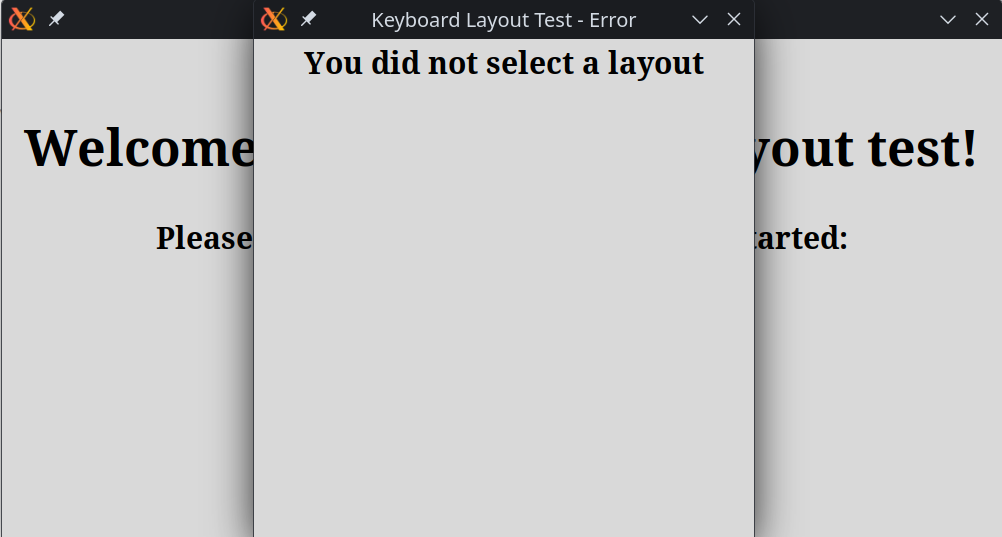
\includegraphics[width=0.75\linewidth]{Error_Screen.png}
        \caption{Error window}
        \label{fig:enter-label}
    \end{figure}

    If the user does not select a layout, an "error window" displays a message. This leaves the starting window open, allowing the user to exit the error window and return to select a layout without exiting the program.

    \begin{figure}[H]
        \centering
        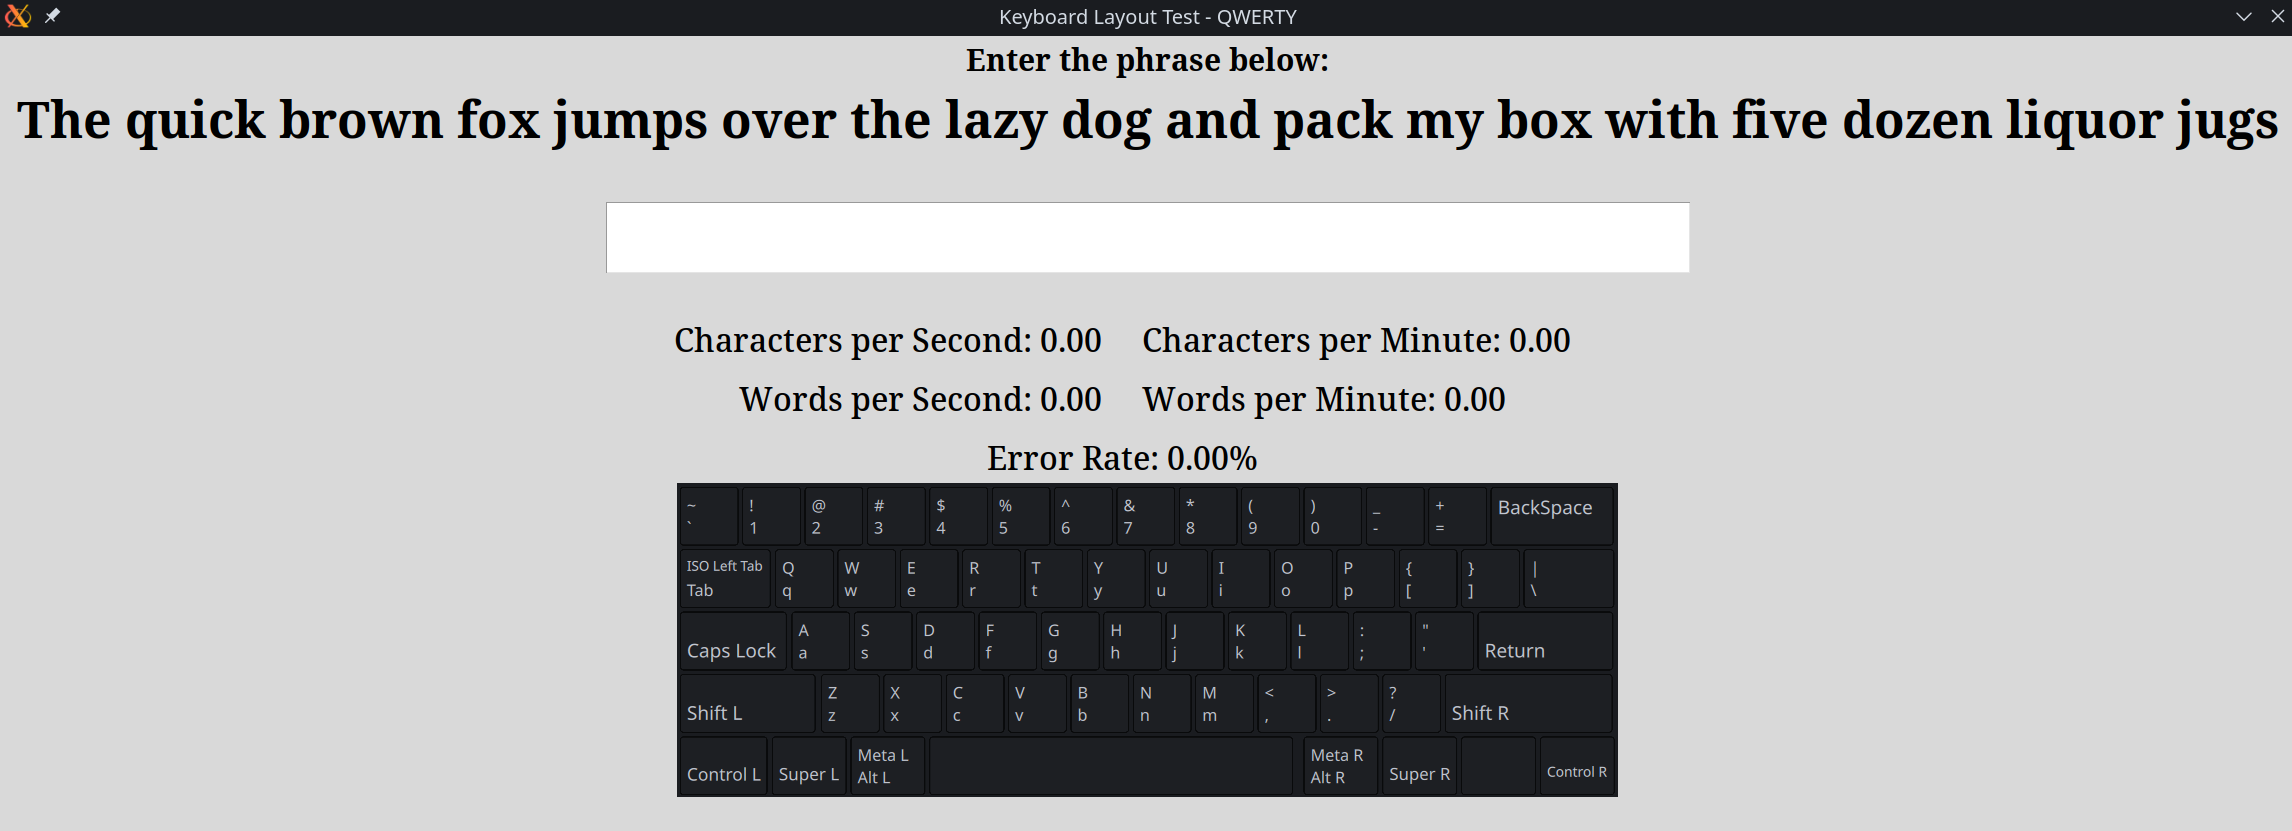
\includegraphics[width=0.75\linewidth]{QWERTY.png}
        \caption{QWERTY keyboard layout}
        \label{fig:enter-label}
    \end{figure}

    The QWERTY keyboard layout is the control group of participants to which other layout statistics will be compared.

    \begin{figure}[h]
        \centering
        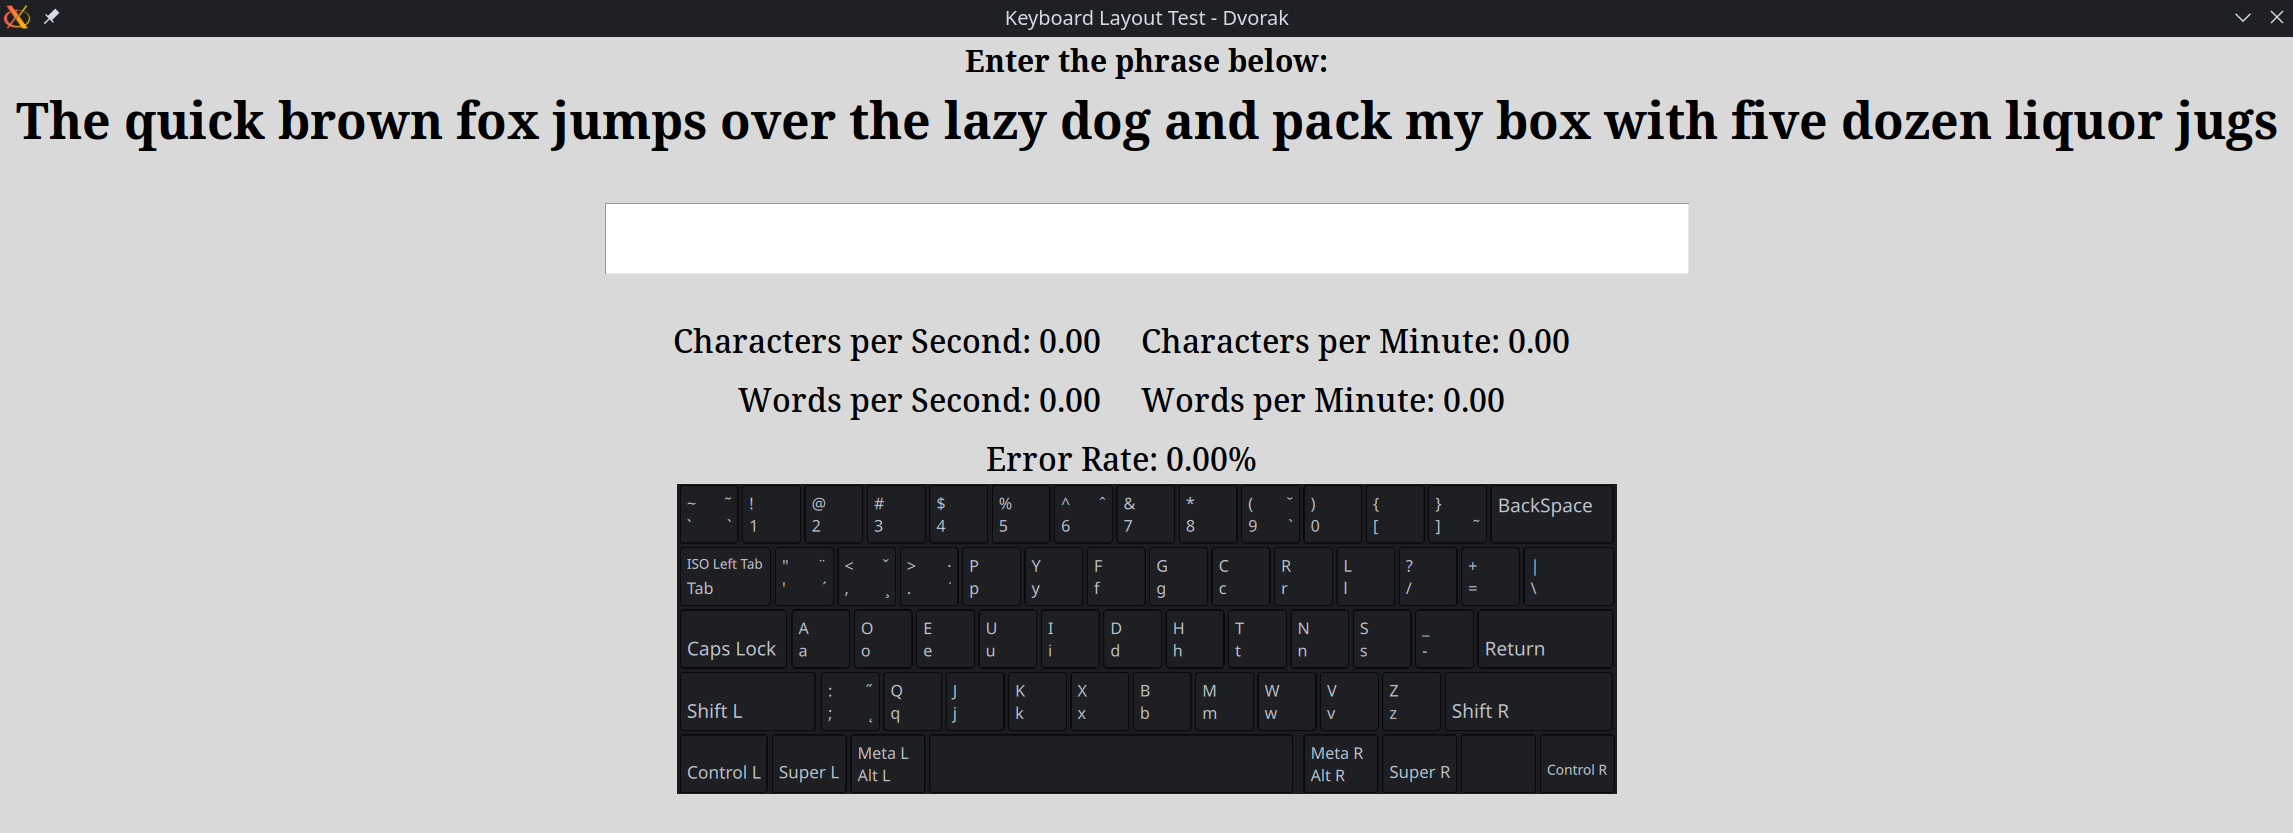
\includegraphics[width=0.75\linewidth]{Dvorak.png}
        \caption{Enter Caption}
        \label{fig:enter-label}
    \end{figure}

    The Dvorak keyboard layout increases typing speed[18] and accuracy while reducing typing effort. It is designed with the most commonly used keys on the right side, which receives about 56 percent of input from the right hand, compared to QWERTY, which receives about 56 percent of input from the left hand. As most people are right-handed, using the Dvorak keyboard may lead to even more significant speed and accuracy over time.


    \begin{figure}[H]
        \centering
        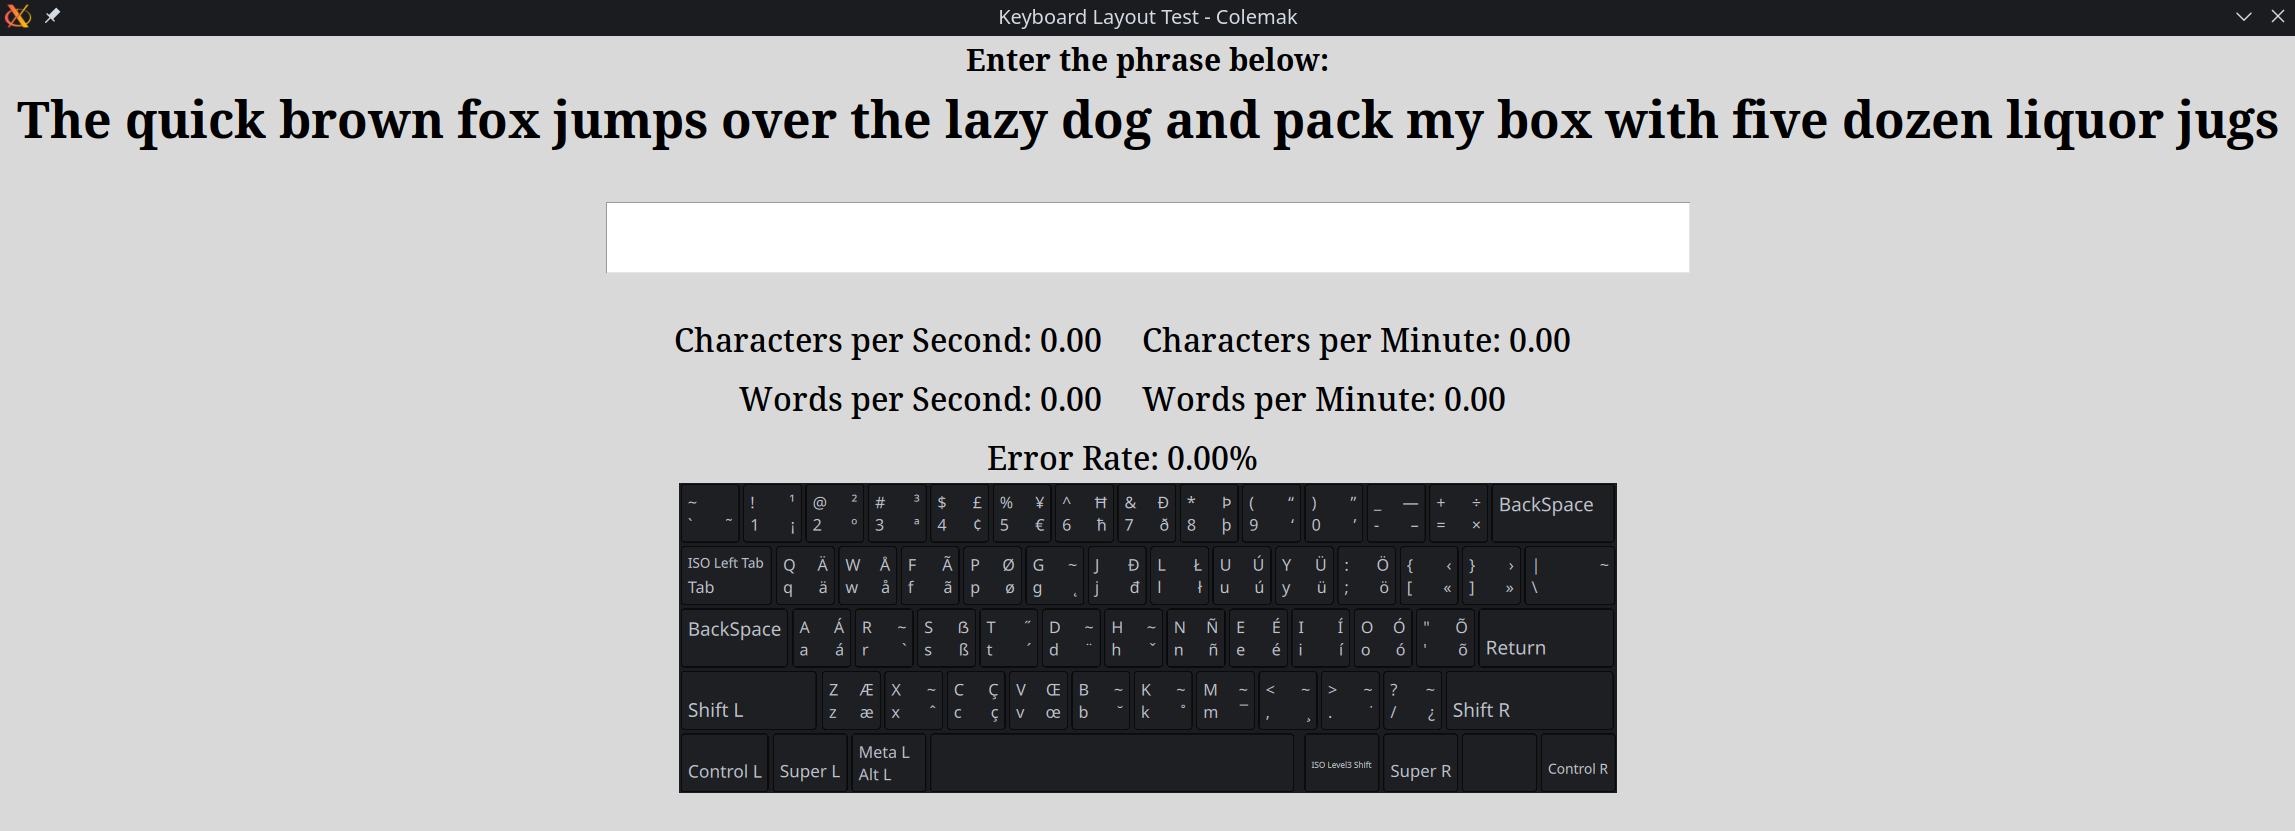
\includegraphics[width=0.75\linewidth]{Colemak.png}
        \caption{Enter Caption}
        \label{fig:enter-label}
    \end{figure}

    The Colemak keyboard layout is designed to be upgraded to Dvorak while being more similar to the QWERTY layout. It also utilizes the right hand more than QWERTY but less than Dvorak.


    \begin{figure}[H]
        \centering
        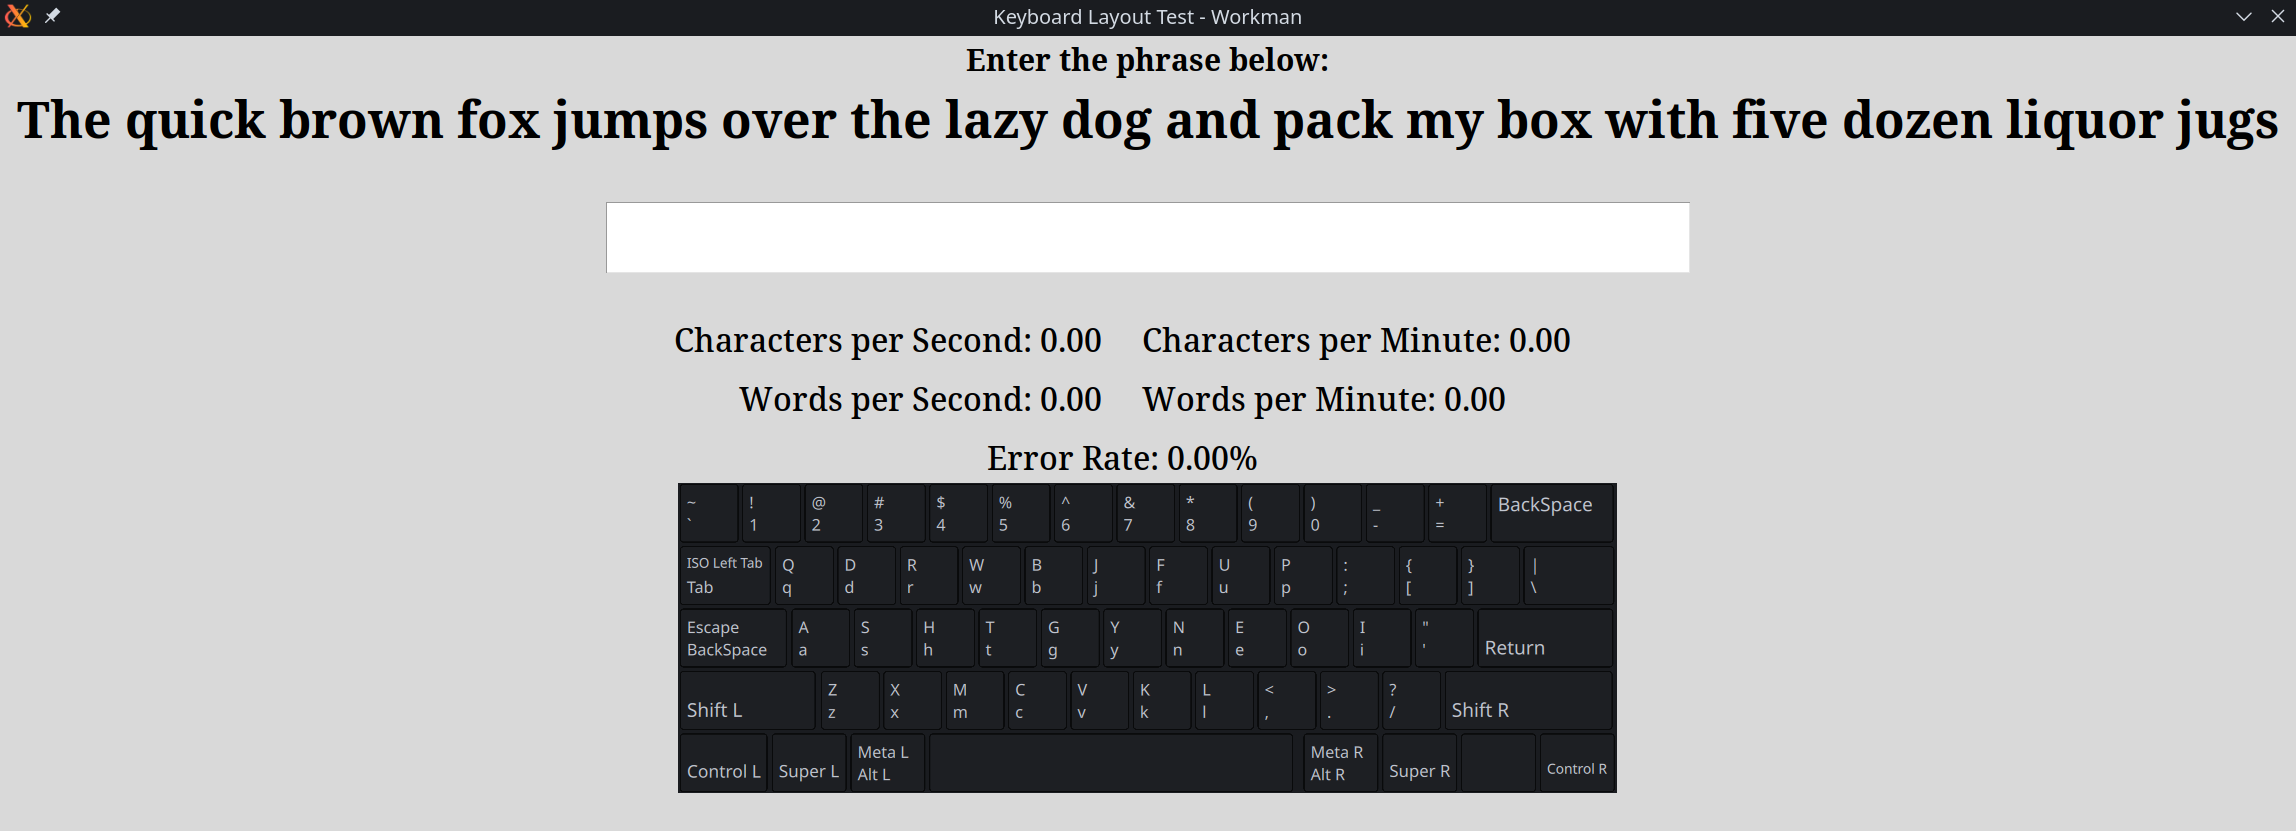
\includegraphics[width=0.75\linewidth]{Workman.png}
        \caption{Enter Caption}
        \label{fig:enter-label}
    \end{figure}

    The Workman keyboard layout is designed to be ergonomic, with about fifty percent of the input coming from each hand. The most commonly used keys are placed comfortably within the fingers' range of motion, which may be more viable for long-term use.

    \begin{figure}[H]
        \centering
        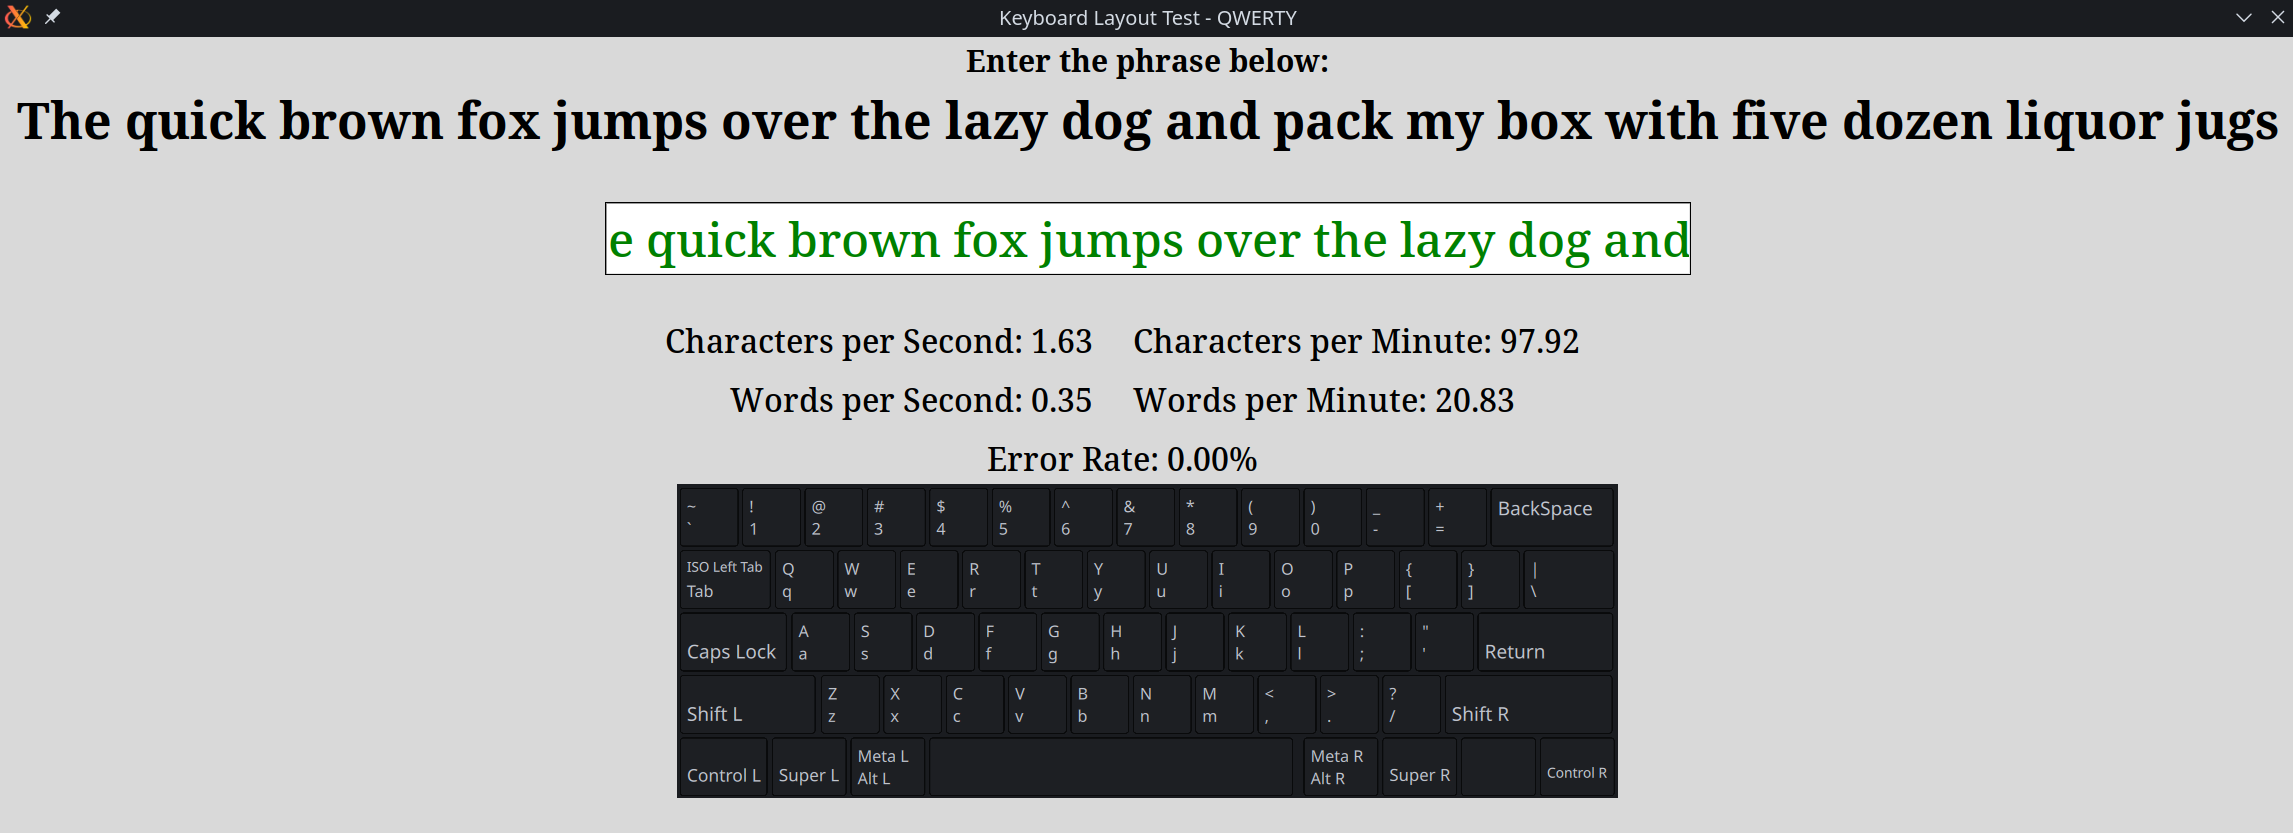
\includegraphics[width=0.75\linewidth]{greenText.png}
        \caption{Correct Text}
        \label{fig:enter-label}
    \end{figure}

    The green text will notify the user that they have correctly typed the phrase until the current point.
    
    \begin{figure}[H]
        \centering
        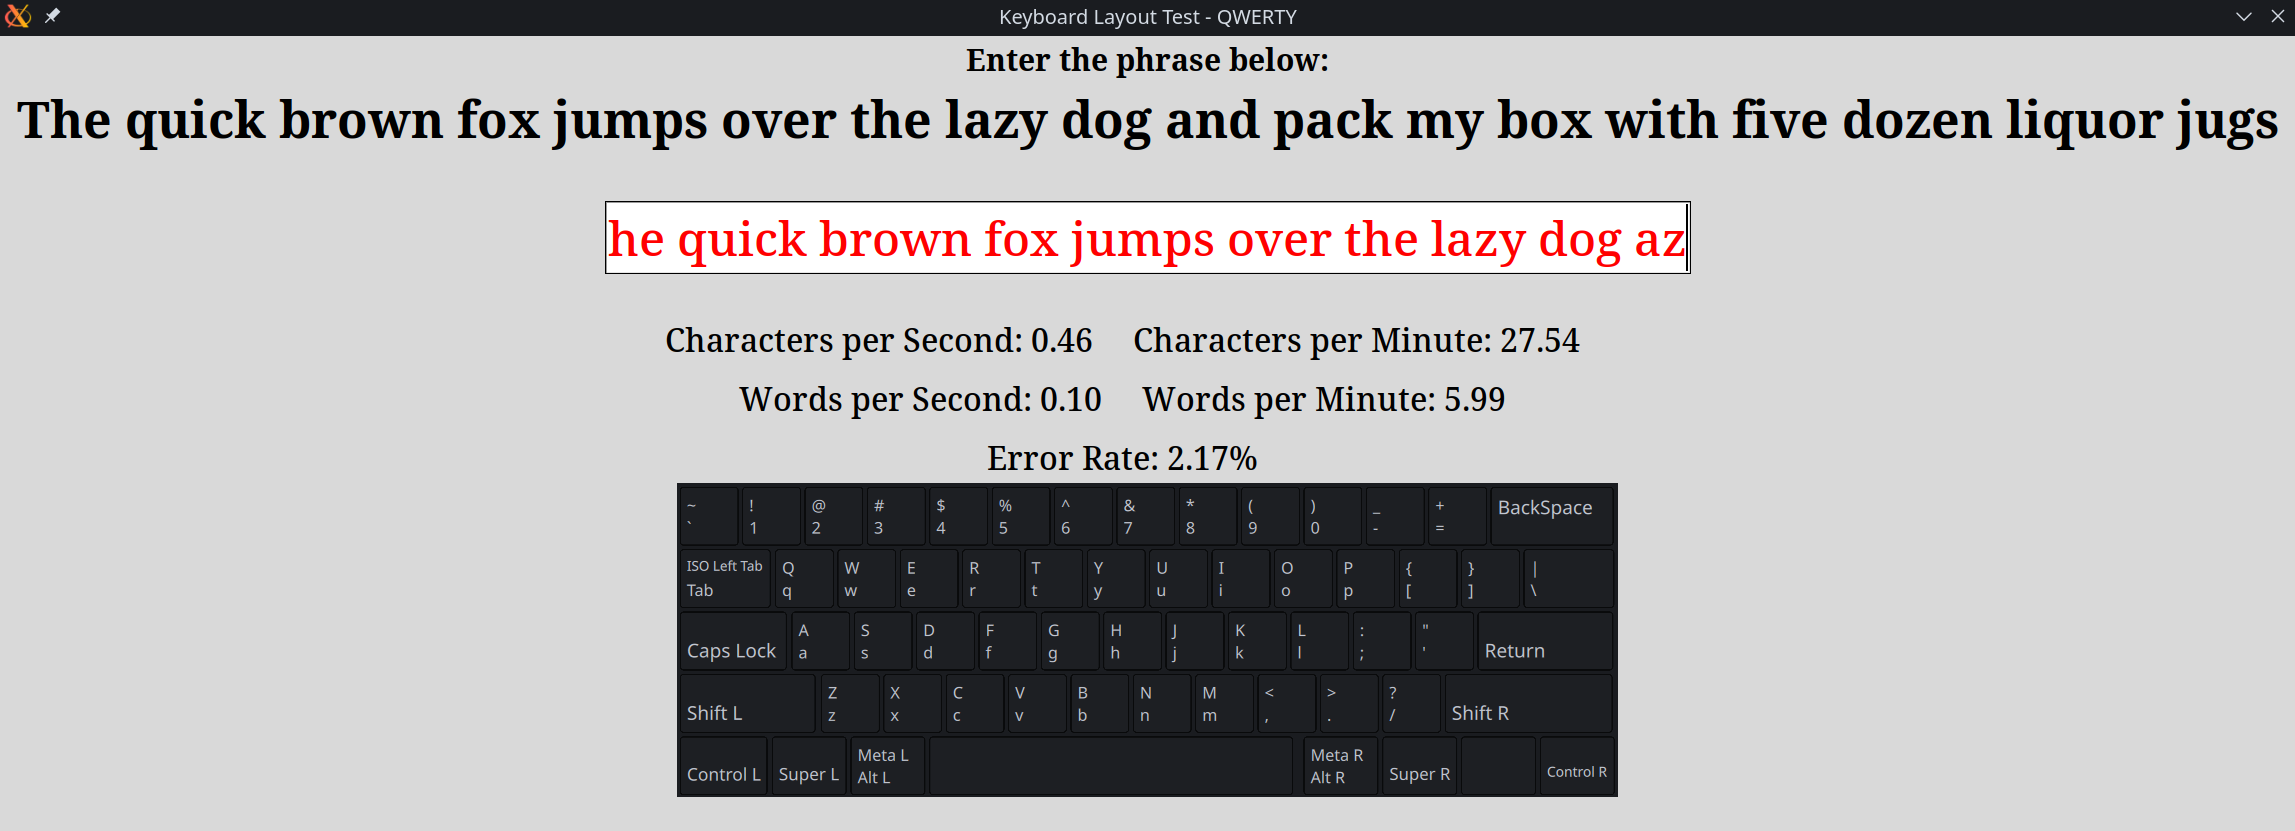
\includegraphics[width=0.75\linewidth]{redText.png}
        \caption{Error Text}
        \label{fig:enter-label}
    \end{figure}

    The red text will notify the user that they have made an error on the last character inputted.
    
    \begin{figure}[H]
        \centering
        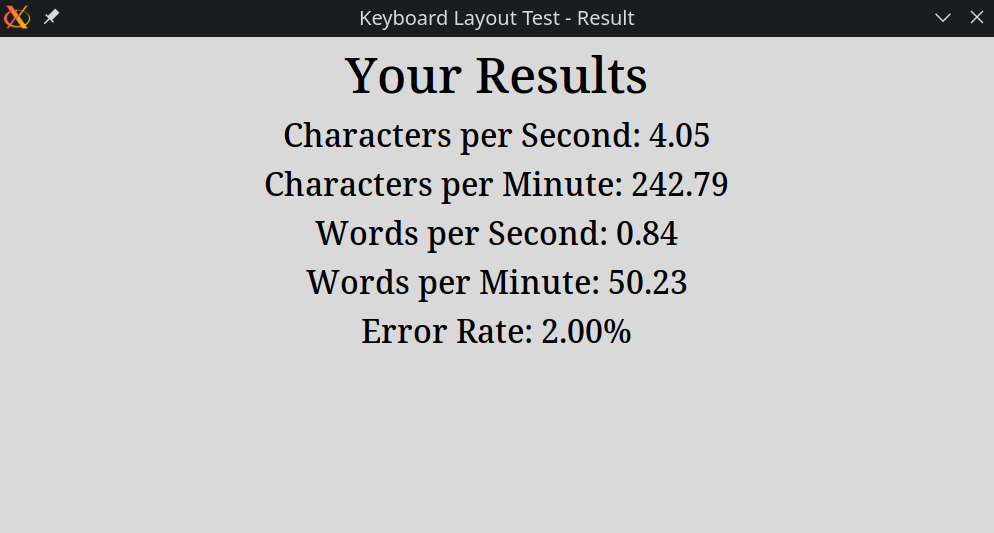
\includegraphics[width=0.75\linewidth]{testResults.png}
        \caption{Test Results}
        \label{fig:enter-label}
    \end{figure}

    The result screen shows the participant's words per minute and other statistics for the test.

    \subsection{Experiment Design}

    This experiment utilizes the typing test application and a mechanical keyboard with modified key cap positions to match the tested layout. The typing test starts with selecting a layout, which the experimenter will set based on the participant's group. During the test, the participant can see their words per minute and other statistics are updated live as they complete the test. Other statistics consist of words per second, characters per second, and characters per minute. The test starts with displaying the phrase "The quick brown fox jumped over the lazy dog and pack my box with five dozen liquor jugs, " a combination of two pangrams, meaning all letters are used at least once. The test finishes and exits to the result screen when the entire phrase is correct. The program will then display a window with the participants' words per minute and other statistics. Sixteen participants, most of whom are college students aged between eighteen and twenty-five, at Colorado State University and a few from other nearby universities, were recruited for the experiment, with four participants for each layout. Each participant was given a consent form to sign, agreeing to allow us to conduct the experiment on them and use the data we collected. The participants were given one practice test to get familiar with the keyboard layout and the program. The participants then completed the test five times with a single layout. After completing the experiment, the participants are asked to complete a questionnaire with feedback from their experience. The results from each trial are collected and examined for improvement and the highest speed and accuracy.

\section{Results and Discussion}
    \subsection{Experiment Results}
        The results of the physical keyboard layout experiment showed that the QWERTY keyboard layout's average words per minute were far higher than the other layouts. Participants using alternative layouts mainly relied on a visual search to find the keys to press, which caused much slower times compared to QWERTY. Most of these participants occasionally defaulted to muscle memory, which caused errors and led to slower results. The Colemak layout had the second-highest average words per minute, with the Workman layout coming in third, and the Dvorak layout had the lowest average words per minute. The words per minute are calculated by dividing the number of words typed by the time elapsed. The results also include words per second, characters per second, and characters per minute. Still, they are excluded from our findings since they are less significant and contribute to the main words per minute calculation.
    \subsection{Result analysis}
        The results of the experiment below show that the average words per minute over all trials for the QWERTY layout average words per minute is 70.939, 4.877 words per minute for the Dvorak layout, 7.581 words per minute for the Colemak layout, and 7.278 words per minute for the Workman layout.
        
            \begin{figure}[H]
                \centering
                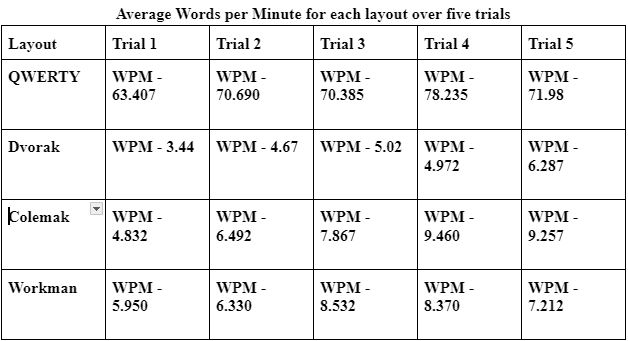
\includegraphics[width=0.75\linewidth]{464 avg data.JPG}
                \caption{Data table for words per minute of each trial}
                \label{fig:enter-label}
            \end{figure}

        The QWERTY layout results slightly improve over a few trials as the participant warms up to type. This average remains similar throughout all trials, with slight deviations due to an outlier on the quicker and slower ends. As expected, the average of the other keyboard layouts was nowhere close to the QWERTY layout, but there were improvements over several trials. The Colemak layout had an average increase for each trial of 1.106 words per minute, the Dvorak layout had an average increase of 0.711 words per minute, and Workman had an average increase of 0.315 words per minute. Of the non-QWERTY layouts, this gives the Colemak layout the highest average increase in words per minute after each trial. Surprisingly, the Dvorak layout had the second-highest average increase, with the Workman layout having the lowest average improvement. However, this was due to the Workman layout's higher average and consistency across all trials. These results show that the Colemak layout is the most viable for replacing the standard QWERTY layout, given enough time to learn. This is due to improved ergonomics, efficiency, and similarities in layouts, decreasing the learning curve. Dvorak would be the second most viable standard layout due to its optimization over the QWERTY layout, but it would take the longest to learn. Although Workman had the initial highest words per minute due to its improved ergonomics over the other layouts, the low average increase makes it undesirable for the most efficient typing. Through the experimenter's observations, the Dvorak layout participants had the least enjoyment throughout the trials, while the Colemak layout had the least negative user responses. Overall, the Colemak layout provides the best of both worlds by increasing ergonomics and efficiency from the QWERTY layout while being similar enough not to be a hassle to learn. 
    \subsection{Post-Experiment Questionnaire Results}
        In the post-experiment questionnaire that participants were asked to complete, feedback was gathered on which layout the participant used if they did not use the QWERTY layout, if they would use that layout again, and the difficulty level between one and five of the layouts used compared to the QWERTY layout. Besides the difficulties with alternative keyboard layouts, the other biggest complaint was the experiment taking too long due to the length of the phrase. The participants who used the QWERTY layout were asked if they would consider using any other layout. Most participants said no, while some said they would consider trying other layouts but would not permanently switch over. Every participant using the Dvorak layout reported the highest difficulty level at five and would not use it again. The responses for the Colemak and Workman layouts reported similar difficulties at ratings of three for the more experienced typists and a rating of four for the rest. Although most of these participants would not use their tested layout again. Some participants said they would consider learning and using Colemak and Workman for fun or specific situations but never as their main keyboard layout.
        

    \subsection{Issues and Limitations}
        Throughout the experiment process, several hurdles prevented the completion of results. By acknowledging these problems, future research can improve on and avoid the same mistakes. The biggest hurdle is the error rate statistic, which is not included in the findings due to faulty calculations in the application, which did not calculate repeated errors in an attempt to fix others. The other big hurdle was having two experimenters conduct the experiment individually using different hardware. Although this may not seem significant since the test run is still the same, the results may have been more accurate and consistent had all experiments been run on the same hardware. Even so, the results are mostly accurate due to verification from testing the application results against other speed typing applications before beginning experimentation. Due to time constraints during experimentation, only sixteen participants were gathered rather than the planned twenty to keep group sizes even. In future research, ensuring that all results are calculated correctly and potentially having more participants gather more data based on the research method will lead to improved research.
\section{Conclusion}
    After experimenting with physical keyboards and modifying their layouts to alternative Dvorak, Colemak, and Workman layouts, we find that the Colemak layout is the most viable replacement to the QWERTY layout, research has shown this even in typing non-English languages[20]. While the Dvorak has the potential to be faster than QWERTY, and the Workman is made purely for ergonomics, they do one thing and one thing well. The Colemak keyboard provides the best of both worlds by creating a layout that improves the efficiency and ergonomics of QWERTY, which was not designed to be ergonomic. All of this is achieved while maintaining the most similarity to QWERTY compared to other alternative layouts. While these are just the findings regarding this experiment, the question still remains of which keyboard layout is truly the best. More layouts may be created in the future. Further research is needed to confirm whether the Colemak layout is the best alternative or if another keyboard layout is more optimal.
\section{Acknowledgments}
    The authors would like to thank Dr. Francisco Ortega, Richi Rodriguez, and Ethan Holen from Colorado State University, without whom this research and experiment would not have come to fruition. Their assistance and feedback allowed us to further our research in an often-overlooked area. We also extend our gratitude to those who gave our group the time of day to participate in our experiment, without whom this research would not have been possible. 
\bibliographystyle{ACM-Reference-Format}
\bibliography{sample-base}

[1]$Ciobanu, O., Gavat, C., \& Cozmei, R. (2015b). The keyboard remains the least ergonomically designed computer device. 2015 E-Health and Bioengineering Conference (EHB). https://doi.org/10.1109/ehb.2015.7391585 
$

[2]$Oladeinde, \& Diagboya. (n.d.). PERFORMANCE EVALUATION OF THREE COMPUTER KEYBOARD LAYOUTS FOR NOVICE TYPISTS. JCESE. https://j-cese.com/storage/app/public/Sh5jkaGpEbF2YzaGmgc5i446Si1eP0ABjz8dj3lZ.pdf 
$

[3]$Buzing, P. (2003, July 31). (PDF) comparing different keyboard layouts: Aspects of Qwerty, ... ResearchGate. https://www.researchgate.net/publication/252214871\_Comparing\_Different\_Keyboard\_Layouts\_Aspects\_of\_QWERTY\_DVORAK\_and\_alphabetical\_keyboards
$

[4]$Jokinen, J. P. P., Sarcar, S., Oulasvirta, A., Silpasuwanchai, C., Wang, Z., \& Ren, X. (2017, May). Modelling Learning of New Keyboard Layouts. Modelling learning of new keyboard layouts. https://dl.acm.org/doi/epdf/10.1145/3025453.3025580 
$

[5]$Onsorodi, A. H., \& Korhan, O. (2020). Application of a genetic algorithm to the keyboard layout problem. PLOS ONE, 15(1). https://doi.org/10.1371/journal.pone.0226611 
$

[6]$Neill, S. B. (1980, June). Dvorak vs. Qwerty: Will Tradition Win Again?. JSTOR. https://www.jstor.org/stable/20385687?casa_token=oDNZ3T2Zla8AAAAA\%3A5woXX2cTD2ou6zlenJYSeTdSihMPAJCSQlPeoLO-MX_NvebJ5Rs7Ea3lwl0WSEMclFoewIvhD6jOo60Utqi21amiPHKu4OL\_Ax0xfVwiMsUE5EvzMvIOVQ\&seq=1 
$

[7]$Puka, R., Łebkowski, P., \& Duda, J. (2021). One row keyboard: The concept of designing a common layout for physical and virtual keyboards. Electronics, 10(6), 663. https://doi.org/10.3390/electronics10060663 
$

[8]$Yang, N., \& Mali, A. D. (2016). Modifying keyboard layout to reduce finger-travel distance. 2016 IEEE 28th International Conference on Tools with Artificial Intelligence (ICTAI). https://doi.org/10.1109/ictai.2016.0034 
$

[9]$Francis, D. (n.d.). Dvorak and Colemak keyboards. Digital Commons at Butler University. https://digitalcommons.butler.edu/cgi/viewcontent.cgi?article=5476\&context=wordways 
$

[10]$Durek, M., \& Nakic-Alfirevic, T. (2004). The Dvorak keyboard layout and possibilities of its regional adaptation | IEEE conference publication | IEEE xplore. IEEE Xplore. https://ieeexplore.ieee.org/document/1372435 
$

[11]$Joyce, B., \& Moxley, R. (1989). Moxley, Roy A. Title comparing children’s typing skills ... Education Resources Information Center. https://files.eric.ed.gov/fulltext/ED313002.pdf 
$

[12]$Keyboard Efficiencies Revisited: Direct Measures of Speed on the Dvorak and Standard Keyboards. ProQuest. (1994). https://www.proquest.com/openview/5518f2557c420cdd687fb7c7444e8152/1?cbl=1817376\&pq-origsite=gscholar 
$

[13]$Anderson, A. M., Mirka, G. A., \& Joines, S. M. (2007). Learning rate analysis of alternative keyboards. PsycEXTRA Dataset. https://doi.org/10.1037/e577952012-003 
$

[14]$Piepgrass, D. (n.d.). Why QWERTY, And What’s Better? CiteSeer. https://citeseerx.ist.psu.edu/document?repid=rep1\&type=pdf\&doi=3206c1a3845fcf49ec5592149caf4776f2772ee1 
$

[15]$West, L. (n.d.). The Standard and Dvorak Keyboards Revisited: Direct Measures of Speed. CiteSeerX. https://citeseerx.ist.psu.edu/document?repid=rep1\&type=pdf\&doi=4d330c3663653842c1623579309f8949b49cb780 
$

[16]$Land, R. I. (1981). Keyboard entry - can it be simplified? ACM SIGSOC Bulletin, 13(2–3), 53–58. https://doi.org/10.1145/1015579.810962 
$

[17]$Shieh, K.-K., \& Lin, C.-C. (1999). A quantitative model for designing keyboard layout. Perceptual and Motor Skills, 88(1), 113–125. https://doi.org/10.2466/pms.1999.88.1.113 
$

[18]$Walker,C. P. (2003, December 5). Evolving a more optimal keyboard. CiteSeer. https://citeseerx.ist.psu.edu/document?repid=rep1\&type=pdf\&doi=11bc0b2409090f7fab4676102f581ff53057b51a 
$

[19]$Hiraga, Y., Ono, Y., \& Yamada-Hisao. (1980). An analysis of the standard English keyboard. Proceedings of the 8th Conference on Computational Linguistics  -. https://doi.org/10.3115/990174.990218
$


[20]$Salvo, J. M., Raagas, C. J., Medina, M. T., \& Portus, A. J. (2016). Ergonomic keyboard layout designed for the Filipino language. Advances in Intelligent Systems and Computing, 407–416. https://doi.org/10.1007/978-3-319-41694-6_41 
$

\end{document}
\endinput
%%
%% End of file `CS464_Final_Report.tex.'